\section{MgNet: a new network structure}\label{sec:mgnet}
In this section, we introduce a new neural network structure,
named as MgNet, motivated by the multigrid algorithm, 
Algorithm \ref{alg:L-Slash0}, as discussed in the previous section.

%The main structure of both CNN and multigrid can be 
%understood as:
%\begin{itemize}
%	\item Solving an undetermined system in grid $\ell$.
%	\item Connection of different grids by restriction and prolongation.
%\end{itemize}

First, given the data-feature equation \eqref{Auf}, we consider
its restrictions to grid $\ell$ as follows:
\begin{equation}
\label{Auf-ell}
A^\ell(u^\ell) = f^\ell, \quad \ell=1:J,
\end{equation}
where
\begin{equation}
\label{f-ell}
f^{\ell}\in\mathbb R^{m_\ell\times n_\ell\times c_\ell},
\end{equation}
and 
\begin{equation}
\label{u-ell}
u^{\ell}\in\mathbb R^{m_\ell\times n_\ell\times h_\ell}.
\end{equation}
We are now in a position to state the main algorithm, namely
MgNet as:
\begin{breakablealgorithm}
	\caption{$u^J={\rm MgNet}(f; J,\nu_1, \cdots, \nu_J)$}
	\label{alg:mgnet}
	\begin{algorithmic}
		\State Initialization:  $f^1 =\theta(f)$, $u^{1,0}=0$
		%		\State Initialization $u^{1,0}$
		\For{$\ell = 1:J$}
		\For{$i = 1:\nu_\ell$}
		\State Feature extraction (smoothing):
		\begin{equation}\label{mgnet}
		u^{\ell,i} = u^{\ell,i-1} + B^{\ell,i}  ({f^\ell -  A^{\ell} (u^{\ell,i-1})}).
		\end{equation}
		\EndFor
		\State Note: 
		$
		u^\ell= u^{\ell,\nu_\ell} 
		$
		\State Interpolation and restriction:
		\begin{equation}
		\label{interpolation}
		u^{\ell+1,0} = \Pi_\ell^{\ell+1}u^{\ell}
		\end{equation}
		\begin{equation}
		\label{restrict-f}
		f^{\ell+1} = R^{\ell+1}_\ell(f^\ell - A^\ell(u^{\ell})) + A^{\ell+1} (u^{\ell+1,0}).
		\end{equation}
		\EndFor
	\end{algorithmic}
\end{breakablealgorithm}

The first property of MgNet is that it recovers the multigrid methods.
\begin{theorem}
	If $A^\ell$, $R_\ell^{\ell+1}$ and $B^{\ell,i} = S^{\ell}$ are all linear operations as described in multigrid method
	in \S \ref{sec:mg}. 
	Then Algorithm \ref{alg:L-Slash0} is equivalent to Algorithm \ref{alg:mgnet} with any choice of $\Pi_\ell^{\ell+1}$.
\end{theorem}
\begin{proof}
	Here we replace $u^{\ell,i}$ and $f^{\ell}$ by $\tilde u^{\ell,i}$ and $\tilde f^{\ell}$ in MgNet. 
	What we want to prove are
	\begin{equation}\label{eq:f-u}
	\tilde f^{\ell} =  f^{\ell} + A_\ell \tilde u^{\ell,0} \quad \text{and} \quad u^{\ell,i} = \tilde u^{\ell, i} - \tilde u^{\ell, 0},
	\end{equation}
	with $u^{\ell,i}$, $f^\ell$ in Algorithm \ref{alg:L-Slash0} and 
	$\tilde u^{\ell,i}$, $\tilde f^\ell$ in Algorithm \ref{alg:mgnet} for any choice of $\Pi_\ell^{\ell+1}$. 
	We prove this result by induction. 
	\begin{itemize}
		\item It is easy to check that $\ell = 1$ is right by taking $\theta  = \rm{id}$. 
		\item Once the above equation \eqref{eq:f-u} is right for $\ell$, 
		let us prove the corresponded result for $\ell+1$.
		\begin{itemize}
			\item For $\tilde f^{\ell+1}$, as the definition in Algorithm \ref{alg:mgnet}, we have
			\begin{align*}
			\tilde f^{\ell+1} &= R_\ell^{\ell+1}(\tilde f^\ell - A^\ell \tilde u^{\ell,\nu_\ell}) + A^{\ell+1}\tilde u^{\ell+1,0}, \\
			&= R_\ell^{\ell+1}(\tilde f^\ell + A^{\ell} \tilde u^{\ell,0}- A^{\ell} \tilde u^{\ell,\nu_\ell}) + A^{\ell+1}\tilde u^{\ell+1,0} \\
			&= R_\ell^{\ell+1}(\tilde f^\ell - A^{\ell} (\tilde u^{\ell,\nu_\ell}- u^{\ell,0})) + A^{\ell+1}\tilde u^{\ell+1,0} \\
			&= R_\ell^{\ell+1}(f^\ell - A^{\ell} u^{\ell,\nu_\ell}) + A^{\ell+1}\tilde u^{\ell+1,0}, \\
			&=  f^{\ell+1} + A^{\ell+1}\tilde u^{\ell+1,0}.
			\end{align*}
			\item For $u^{\ell+1,i}$, first we have 
			$$
			u^{\ell+1,0} = 0 =\tilde u^{\ell+1, 0} - \tilde u^{\ell+1, 0},
			$$
			then we prove 
			\begin{equation}\label{u:i+1}
			u^{\ell+1,i} = \tilde u^{\ell+1, i} - \tilde u^{\ell+1, 0}
			\end{equation} by induction for $i$.
	
			We assume \eqref{u:i+1} holds for $0,1,\cdots,i-1$. Let us miner $\tilde u^{\ell+1, 0}$ in both sides of 
			the smoothing process \eqref{mgnet} in Algorithm \ref{alg:mgnet}. Then we have
			\begin{align*}
			\tilde u^{\ell+1,i} - \tilde u^{\ell+1, 0} &= \tilde u^{\ell+1,i-1} - \tilde u^{\ell+1, 0} + B^{\ell+1,i} (\tilde f^{\ell+1} - A^{\ell+1} \tilde u^{\ell+1,i-1}), \\
			&= \tilde u^{\ell+1,i-1} - \tilde u^{\ell+1, 0} + B^{\ell+1,i} (f^{\ell+1} + A^{\ell+1}\tilde u^{\ell+1,0} - A^{\ell+1} \tilde u^{\ell+1,i-1} ),\\ 
			&= u^{\ell+1,i-1} + B^{\ell+1,i} (f^{\ell+1} - A^{\ell+1}u^{\ell+1,i-1} ).
			\end{align*}
			This is exact the smoothing process in Algorithm \ref{alg:L-Slash0} as we take $ B^{\ell+1,i} = S^{\ell+1}$.
			%			\item At last, recall that $u^{1,0} = 0$, so the output of Algorithm \ref{alg:L-Slash0} 
			%			$$
			%			tilde u^{1, \nu_1} = u^{1, \nu_1},
			%			$$
			%			which is the output of Algorithm \ref{alg:L-Slash}. 
		\end{itemize}
	\end{itemize}
\end{proof}

Despite of the simplicity look of Algorithm \ref{alg:mgnet}, there
are rich mathematical structures and variants which we briefly discuss below.

\subsection{Initialization: feature space channels}
Initially for $\ell=1$,  we take $m_1 = m$ and $n_1 = n$ and we may define the linear mapping 
\begin{equation}
\label{eq:6}
\theta: \mathbb R^{m\times n\times c}
\mapsto \mathbb R^{m_1\times n_1\times c_1},
\end{equation}
to obtain $f^{1} = \theta(f)$ with $c$ given in \eqref{data-c} changed to the channel of the initial
data space to $c_1$.   Usually
\begin{equation}
\label{cc}
c_1\ge c.  
\end{equation}
One possibility is that we choose $c_1=c$.  In this case, we choose
$\theta=$identity.   But in general, we may need to choose $c_1\gg
c$. One possible advantage of preprocessing the RGB ($c=3$) to 
different color spaces is that we can better choose what kind of
features the CNN can detect, and under what 
conditions those detections will be invariant.

One possibility of understanding and modifying this step 
is to decompose the data $f$ into a number of more
specialized data
\begin{equation}
\label{decomp-f}
f=\sum_{k=1}^{c_1}\xi_kf^1_k  =\xi^Tf^1.
\end{equation}
We may use some knowledge from image processing or physics to
design a procedure to obtain the right decomposition of
\eqref{decomp-f}, or we can just train it. 
Conceivably, we may view $f^{1} = \theta(f)$ as a special approximation solution of
\eqref{decomp-f} with the same sparsity pattern to $\xi$. 

\subsection{Extracted Units: $u^{\ell}$ and channels}
The first new feature and the main new ingredient 
in the proposed neural network is the introduction 
of feature variables  $u^{\ell}$ in \eqref{u-ell}, which will be known
as the extracted units. 

We emphasize that the extracted-units $u^\ell$ and the data $f^\ell$ can have
different numbers of channels:\
\begin{equation}
\label{uf-channels}
u^\ell\in \mathbb{R}^{m_\ell\times n_\ell \times c_{u,\ell}}, \quad
f^\ell\in \mathbb{R}^{m_\ell\times n_\ell \times c_{f,\ell} }
\end{equation}
One possibility is that the number of channels for both $u$ and $f$ remain
unchanged in different grids:  
\begin{equation}
\label{cfl}
c_{f,\ell}=c_f, \quad \ell=1:J,   
\end{equation}
and 
\begin{equation}
\label{ufl}
c_{u,\ell}=c_{u}, \quad \ell=1:J.   
\end{equation}
Both $c_f$ and $c_{u}$ are two super-parameters that need to be tuned, 
and we may even take $c_u = c_f$.

\subsection{Poolings: $\Pi_{\ell+1}^\ell$ and $R_{\ell+1}^\ell$}
The pooling $\Pi_{\ell+1}^\ell$ in \eqref{restriction} and
$R_{\ell+1}^\ell$ in \eqref{restrict-f} are in general different.
They can be trained in general, but they may be a priori chosen.

There are many different possibilities to choose $\Pi_{\ell+1}^\ell$. 
The simplest choice of $\Pi_{\ell+1}^\ell$ is 
\begin{equation}
\label{eq:8}
\Pi_{\ell+1}^\ell=0.
\end{equation}
A more sophisticated choice can be obtained by considering an
interpolation from fine grid to coarse (that, for example preserves linear function
locally).  Namely
\begin{equation}
\label{Pi}
\Pi_{\ell+1}^\ell=\bar\Pi_{\ell+1}^\ell \otimes I_{c_\ell\times c_\ell} 
\end{equation}
with $\bar\Pi_{\ell+1}^\ell$ given by~\eqref{mg-Pi}.



\subsection{Data-feature mapping: $A^{\ell}$}
The second new feature of MgNet is that this data-feature mapping
only depends on the grid ${\cal T}_\ell$, and it does not depend on layers
within the same grid.  This amounts to a significant saving of the number of
parameters.  In comparison, the existing CNN, such as ResNet, can be
interpreted as a network related to the case that $A^{\ell}$ is
replaced by $A^{\ell, i}$, namely
\begin{equation}\label{u-resnet}
u^{\ell,i} = u^{\ell,i-1} + B^{\ell,i}  (f^\ell -  A^{\ell,i} (u^{\ell,i-1}).
\end{equation}

The data-feature mapping: $A^{\ell}$ can be either linear
\eqref{linearA}, or nonlinear \eqref{nonlinearA}.  The underlying
convolution kernels can be different on different grids and they can
all be trained.


\subsection{Feature extractors: $B^{\ell,i}$}
There are some freedoms in choosing these feature extrators.  
One common choice of extractors is given by \eqref{extractor}, namely 
\begin{equation}
\label{extractor-ell}
B^{\ell,i}=\sigma\circ \eta^{\ell,i}\circ\sigma.
\end{equation}

Other than the level dependent extractors, the following 
different strategies can be used
\begin{description}
	\item[Constant Extractors]: $B^{\ell,i}=B^{\ell}$ for   $i=1:\nu_\ell$
	\item[Scaled Extractors]:$B^{\ell,i}=\alpha_iB^{\ell}$ for   $i=1:\nu_\ell$
	\item[Variable Extractors]: $B^{\ell,i}$
\end{description}



This brief framework gives us the basic principle on designing 
a CNN models for classification. All models are seen as the special
choice of data-feature mapping $A^\ell$, feature extractors $B^{\ell,i}$ 
and the pooling operators $\Pi_{\ell+1}^\ell$ with $R_{\ell+1}^\ell$.


\section{Some classic CNN models}\label{sec:CNNs}
In this section, we will use the notation introduced above to 
give a brief description of some classic CNN models.

\subsection{LeNet-5, AlexNet and VGG}
The  LeNet-5 \cite{lecun1998gradient}, AlexNet \cite{krizhevsky2012imagenet} and VGG \cite{simonyan2014very}
can be written as:
	\begin{equation}
	\begin{cases}
	f^{1,0} &= \theta^0(f), \\
	f^{\ell,i} &= \theta^{\ell,i} \circ \sigma (f^{\ell, j-1}), \quad i = 1:\nu_\ell ~\text{and}~ \ell = 1:J,\\
	f^{\ell+1,0} &= R_\ell^{\ell+1}( f^{\ell,m+\ell}).  \\
	\end{cases}
	\end{equation}
	where $R_\ell^{\ell+1}$ can be general pooling operators and $\theta^{\ell,i}$ can be convolution with stride 1, 
	or fully connected operators.  
	Then the CNN model will be defined by
	\begin{equation}\label{eq:cnndefine}
	H_0(f) = f^{L,\nu_\ell}.
	\end{equation}
	In these three classic CNN models, they still need some 
	extra fully connected layers in nonlinear mapping $H_0$ before the logistic regression as it contains 
	a fully connected layer as in \eqref{eq:log_reg}. 
	These fully connected layers are removed in ResNet to be described below.
\subsection{ResNet}
The ResNet \cite{he2016deep} can be written as
	\begin{equation}\label{ori-ResNet}
	\begin{cases}
	f^{1,0} &=R_{\rm max}\circ \sigma \circ \theta^0(f), \\
	f^{\ell,i} &= \sigma \left( f^{\ell, i-1} + \mathcal{F}^{\ell, i} (f^{\ell,i-1}) \right), \quad i = 1:\nu_\ell ~\text{and}~ \ell = 1:J ,\\
	f^{\ell+1,0} &= \sigma \left( R_\ell^{\ell+1} (f^{\ell, \nu_\ell} )+ \mathcal{F}^{\ell, 0} (f^{\ell, \nu_\ell} ) \right), \quad \ell = 1:J-1,\\
	H_0(f) &=  R_{\rm ave}(f^{L,\nu_\ell}). \\
	\end{cases}
	\end{equation}
	Here
	$$
	\mathcal{F}^{\ell,i} (f^{i-1}) = \xi^{i} \circ \sigma \circ \eta^{i} (f^{i-1}).
	$$
	Generally, $\xi^{\ell,i}$ and $\eta^{\ell,i}$ takes the form of \label{eq:conv-1} with zero padding and stride 1,
	except, $\eta^{\ell,0}$  is taken as convolution with stride 2 with the same output dimension of $R_\ell^{\ell+1}$.
	
\subsection{iResNet} 
	The iResNet\cite{he2016identity} can be written as:
	\begin{equation}\label{eq:iResNet1}
	\begin{cases}
	f^{1,0} &=R_{\rm max}\circ \sigma \circ \theta^0(f), \\
	f^{\ell,i} &= f^{\ell, i-1} + \mathcal{F}^{\ell, i} (f^{\ell,i-1}), \quad i = 1:\nu_\ell ~\text{and}~ \ell = 1:J ,\\
	f^{\ell+1,0} &=  R_\ell^{\ell+1} (f^{\ell, \nu_\ell} )+ \mathcal{F}^{\ell, 0} (f^{\ell, \nu_\ell} ) , \quad \ell = 1:J-1,\\
	H_0(f) &=  R_{\rm ave}(f^{L,\nu_\ell}). \\
	\end{cases}
	\end{equation}
	where
	$$
	\mathcal{F}^{\ell,i} (f^{\ell,i -1}) = \xi^{\ell,i} \circ \sigma \circ \eta^{\ell,i} \sigma (f^{\ell,i-1}).
	$$
	The only difference between ResNet and iResNet can be viewed as 
	putting a $\sigma$ in different places. 
	The connection of those three models are often shown with next diagrams:
	\begin{figure}[!htb]
		\begin{center}
			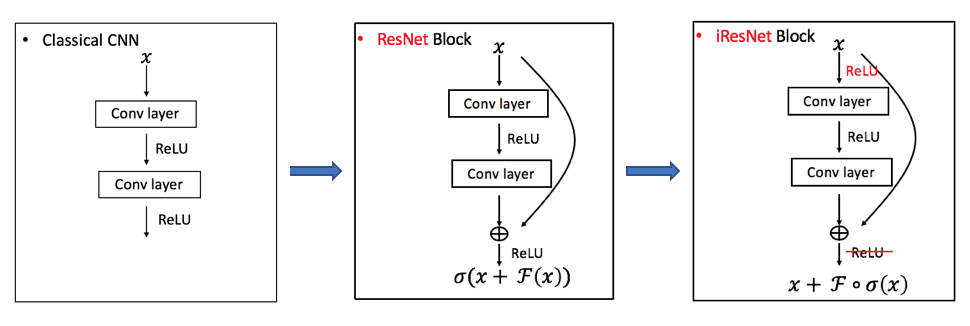
\includegraphics[width=.6\textwidth, height=.13\textheight]{comparison-net} 
		\end{center}
		\caption{Comparison of CNN Structures}
	\end{figure}
	

Without loss of generality, we extract the key 
feedforward steps on the same grid in different CNN models as follows.
\begin{description}
	\item[Classic CNN] 
	\begin{equation}\label{eq:cCNN}
	f^{\ell,i} = \xi^i \circ \sigma (f^{\ell,i-1}) \quad \text{or} \quad f^{\ell,i} = \sigma \circ \xi^{i} (f^{\ell,i-1}) .
	\end{equation}
	\item[ResNet] 
	\begin{equation}\label{eq:ResNet}
	f^{\ell,i} = \sigma( f^{\ell,i-1} + \xi^{\ell,i} \circ \sigma \circ \eta^{\ell,i}(f^{\ell,i-1})).
	\end{equation}
	\item[iResNet]
	\begin{equation}\label{eq:iResNet}
	f^{\ell,i} = f^{\ell,i-1} + \xi^{\ell,i} \circ \sigma \circ \eta^{\ell,i}\circ \sigma(f^{\ell,i-1}).
	\end{equation}
\end{description} 


\section{Variants and generalizations of MgNet}\label{sec:relation}

%\subsection{Some properties of MgNet}
%So, this MgNet is corresponded to the multigrid methods 
%with iteration in function space. A natural idea is that there is also a dual version of 
%MgNet similar with the multigrid methods with iteration in dual space.
The MgNet model algorithm is one very basic and it can be generalized
in many different ways. It can also be used as a guidance to modify and 
extend many existing CNN models. 

The following result show how MgNet is related to he iResNet \cite{he2016identity}. 
\begin{theorem}\label{thm:mgnet1}
The MgNet model Algorithm \ref{alg:mgnet}, 
with $A=\xi^\ell$ and $B^{\ell,i}=\sigma \circ \eta^{\ell,i}\circ\sigma$, 
admits the following identities
\begin{equation}\label{dualmgnet}
f^{\ell, i} = f^{\ell, i-1} -  \xi^{\ell} \circ \sigma \circ \eta^{\ell,i}\circ \sigma (f^{\ell,i-1}), \quad i = 1:\nu_\ell, \\
\end{equation}
where
\begin{equation}
  \label{eq:5}
	f^{\ell,i} = f^{\ell} - \xi^{\ell} (u^{\ell,i}).   
\end{equation}
Furthermore, \eqref{dualmgnet} represents iResNet~\cite{he2016identity} 
as shown in \eqref{eq:iResNet}.
\end{theorem}

\begin{proof}
	Because of the linearity of $\xi^\ell$ and invariant within the same grid $\ell$, 
	we can apply $\xi^\ell$ on both sides of \eqref{mgnet} and minus with
	$f^\ell$, thus we have
	$$
	f^{\ell} - \xi^{\ell} (u^{\ell,i})= f^{\ell} - \xi^\ell(u^{\ell,i}) -
	\xi^{\ell} \circ \sigma \circ \eta^{\ell,i}\circ \sigma (f^\ell + \xi^\ell(u^{\ell,i})).
	$$
This finish the proof with definition in \eqref{eq:5}.
\end{proof}

The above result is very simple but critically important.
In view of Theorem \ref{thm:mgnet1}, it shows how multigrid and 
CNN are intimately related. Furthermore, it provides a different version
of iResNet, which can be viewed as the dual version of the original iResNet.
This relation is quit similar with the dual relation of $u$ and $f$
in multigrid method \cite{xu2017algebraic}.
\begin{lemma}\label{thm:mgnet2} 
	The ResNet~\cite{he2016deep} step
 	 as in \eqref{eq:ResNet} 
%	\begin{equation}\label{resnet}
%	f^{\ell,i} = \sigma( f^{\ell, i-1} - \xi^{\ell,i} \circ \sigma \circ \eta^{\ell,i} (f^{\ell,i-1}) ).
%	\end{equation}
admits the following relation:
%(which resembles closely with \eqref{dualmgnet}) 
\begin{equation}\label{tilde-resnet}
\tilde f^{\ell,i} =\sigma(\tilde f^{\ell,i-1}) -
\xi^{\ell,i} \circ \sigma \circ \eta^{\ell,i}\circ \sigma( \tilde f^{\ell,i-1}),
\end{equation}
where
\begin{equation}\label{tilde-f}
\tilde f^{\ell,i} = f^{\ell, i-1} -\xi^{\ell,i} \circ \sigma \circ \eta^{\ell,i} (f^{\ell,i-1}).
\end{equation}
\end{lemma}
\begin{proof}
%	Now, we will establish the connection between classical ResNet and MgNet. 
	First, we apply $ \xi^{\ell,i+1} \circ \sigma \circ \eta^{\ell,i+1}$ 
	on the both sides of \eqref{eq:ResNet} and get
	\begin{equation}\label{resnet1}
	\xi^{\ell,i+1} \circ \sigma \circ \eta^{\ell,i+1}( f^{\ell,i} ) = 
	\xi^{\ell,i+1} \circ \sigma \circ \eta^{\ell,i+1}\circ \sigma( \tilde f^{\ell,i} ).
	\end{equation}
	Minus by $f^{\ell,i}$ on the both sides and recall the definition in \eqref{tilde-f}, we have
	\begin{equation*}
	\tilde f^{\ell,i+1} = f^{\ell,i} - \xi^{\ell,i+1} \circ \sigma \circ \eta^{\ell,i+1}\circ \sigma( \tilde f^{\ell,i}).
	\end{equation*}
	By the definition of $f^{\ell,i} = \sigma(\tilde f^{\ell,i})$, we finish this proof.
\end{proof}

We call the above form \eqref{tilde-resnet} as
$\sigma$-ResNet, similar to the MgNet we replace $\xi^{\ell,i}$ by $\xi^{\ell}$  and get 
the next Mg-ResNet form as:
\begin{equation}\label{mg-resnet}
f^{\ell,i} =\sigma(f^{\ell,i-1}) -
\xi^{\ell} \circ \sigma \circ \eta^{\ell,i}\circ \sigma(f^{\ell,i-1}).
\end{equation}

If we take these pooling and prolongation operators
as discussed in the previous sections and focus on 
the iterative forms on a certain grid $\ell$, we may
compare them all as:
\begin{table}[!htbp]
	\caption{Comparison for all iterative forms }
	\label{comparison-ALL}
	\begin{center}\scriptsize
		\resizebox{.8\textwidth}{!}{
			\begin{tabular}{|c|c|c|}
				\hline
				Primal-Dual & Model & Iterative form \\
				\hline
				\multirow{3}{*}{Feature space} & Abstract-MgNet & Solving $A^\ell(u^\ell) = f^\ell$ \\
				\cline{2-3}
				& General-MgNet & $u^{\ell,i} = u^{\ell, i-1} + B^{\ell,i} (f^\ell - A^{\ell}(u^{\ell,i-1}))$ \\
				\cline{2-3}
				& {MgNet} & $u^{\ell,i} = u^{\ell, i-1} + \sigma \circ \eta^{\ell,i}\circ \sigma (f^\ell - \xi^{\ell}(u^{\ell,i-1}))$ \\
				\hline
					\multirow{5}{*}{Data space} & iResNet & $ f^{\ell,i} = f^{\ell, i-1} -  \xi^{\ell,i} \circ \sigma \circ \eta^{\ell,i} \circ \sigma (f^{\ell,i-1})$ \\
				\cline{2-3}
				& Mg-iResNet & $f^{\ell,i} = f^{\ell, i-1} -  \xi^{\ell} \circ \sigma \circ \eta^{\ell,i}\circ \sigma (f^{\ell,i-1})$ \\
				\cline{2-3}
				& Mg-ResNet & $f^{\ell,i} = \sigma(f^{\ell,i-1}) - \xi^{\ell} \circ \sigma \circ \eta^{\ell,i}\circ \sigma( f^{\ell,i-1})$ \\
				\cline{2-3}
				& $\sigma$-ResNet & $f^{\ell,i} = \sigma(f^{\ell,i-1}) - \xi^{\ell,i} \circ \sigma \circ \eta^{\ell,i}\circ \sigma( f^{\ell,i-1})$ \\
				\cline{2-3}
				& ResNet & $f^{\ell,i} = \sigma(f^{\ell, i-1} -  \xi^{\ell,i} \circ \sigma \circ \eta^{\ell,i} (f^{\ell,i-1}))$ \\
				\hline
			\end{tabular} 
		}
	\end{center}
\end{table}

We can have these connections for all iterative scheme in data space:
\begin{equation}
\text{ ResNet} \xleftrightarrow{\eqref{tilde-f}} \sigma\text{-ResNet } \xleftrightarrow{\xi^{\ell,i} \leftrightarrow \xi^{\ell}} \text{Mg-ResNet}  
\xleftrightarrow{\sigma(f^{\ell,i-1}) \leftrightarrow f^{\ell, i-1} } \text{Mg-iResNet} \xleftrightarrow{ \xi^{\ell} \leftrightarrow \xi^{\ell,i}} \text{iResNet}.
\end{equation}

%Because of the linearity of $\xi^{\ell,i}$, the above forms of iResNet and ResNet
%are equivalent to the previous as \eqref{dualmgnet} and \eqref{tilde-resnet}.

In this sense, these MgNet related models can be understood as
 models between iResNet and ResNet. And all these models can be
 understood as iteration in the data space as a dual relationship with
 feature space as MgNet.
 
 
The rationality of replacing  $\xi^{\ell,i}$ by layer independent $\xi^{\ell}$ may
be justified by the following theorem. 
\begin{theorem}\label{thm:CNN}
On each grid $\mathcal T_\ell$, 
\begin{enumerate}
	\item Any CNN model with
%	CNN and Mg-ResNet] 
	\begin{equation}
	\label{CNN1}
	f^{\ell,i} =   \chi^{\ell,i} \circ \sigma (f^{\ell,i-1}),
	\end{equation} 
	can be written as
	\begin{equation}\label{Res-CNN1}
	f^{\ell,i} = \sigma(f^{\ell,i-1}) - \xi^{\ell} \circ \sigma \circ \eta^{\ell,i} \circ\sigma ( f^{\ell,i-1}).
	\end{equation}
	\item Any CNN model with 
%	[CNN and ResNet] 
	\begin{equation}
	\label{CNN2}
	f^{\ell,i} =   \sigma\circ\chi^{\ell,i} (f^{\ell,i-1}).
	\end{equation}
	can be written as 
	\begin{equation}\label{Res-CNN2}
	f^{\ell,i} = \sigma\left(f^{\ell,i-1} - \xi^{\ell} \circ \sigma \circ \eta^{\ell,i}  ( f^{\ell,i-1})\right).
	\end{equation}
\end{enumerate}

%\begin{equation}
% \chi^{\ell,i}: \mathbb{R}^{n_\ell \times n_\ell \times c_\ell} 
% \mapsto \mathbb{R}^{n_\ell \times n_\ell \times c_\ell},
%\end{equation}
\end{theorem}
\begin{proof}
%	Without loss of generality, consider the classical CNN with 
%	\begin{equation}
%	f^{\ell,i} =   ({\rm id}  + \tilde \eta^{\ell,i} )\circ \sigma (f^{\ell,i-1}).
%	\end{equation}
Let use prove the first case as an example, 
the second case can be proven with the same process.

With similar structure in MgNet, we can take
\begin{equation}
\label{xi-cnn1}
\xi^{\ell}=  [\hat \delta_1, \cdots, \hat \delta_{{c_\ell}}],
\end{equation}
and 
\begin{equation}
\label{eta-ell}
\eta^{\ell,i} = [{\rm id}_{c_\ell}, -{\rm id}_{c_\ell}] \circ (\chi^{\ell,i} - {\rm id}_{c_\ell}).
\end{equation}
Here 
\begin{equation}
{\rm id}_{c_\ell}: \mathbb{R}^{n_\ell \times n_\ell \times c_\ell} 
\mapsto \mathbb{R}^{n_\ell \times n_\ell \times c_\ell},
\end{equation}
is the identity map and 
\begin{equation}
\hat \delta_k :  \mathbb{R}^{n_\ell \times n_\ell \times 2c_\ell} 
\mapsto \mathbb{R}^{n_\ell \times n_\ell},
\end{equation}
with 
\begin{equation}\label{eq:hatdelta}
\hat \delta_k([X ,Y]) = -([X]_k + [Y]_k),
\end{equation}
for any $X, Y \in \mathbb{R}^{n_\ell \times n_\ell \times c_\ell}$ 
and $[X,Y] \in \mathbb{R}^{n_\ell \times n_\ell \times 2c_\ell} $.


	First, we see that $\eta^{\ell,i}$ with the above 
	form is a convolution from $\mathbb{R}^{n_\ell \times n_\ell \times c_\ell}$
	to  $\mathbb{R}^{n_\ell \times n_\ell \times 2c_\ell}$.
	Following the identity
	\begin{equation}
	ReLU(x) + ReLU(-x) = x,
	\end{equation}
	and the definition of $\xi^{\ell}$ i.e. 
	\begin{equation}
	\xi^{\ell} = \hat \delta,
	\end{equation}
	as a special case in MgNet. 
	For more details, we can give a exact form of 
	$\hat \delta_k$ as in \eqref{eq:hatdelta} with
	\begin{equation}
	\hat \delta_k = [0, \cdots,0, -\delta, \cdots 0;  0, \cdots,0, -\delta, \cdots 0],  \quad k = 1:{c_\ell},
	\end{equation}
	where $\delta$ is the identity kernel during one channel.
	
	At last, we have
	\begin{align}
	\left[\xi^{\ell} \circ \sigma \circ [{\rm id}_{c_\ell}, -{\rm id}_{c_\ell}] (x) \right]_k &=  \left[\xi^{\ell} \circ \sigma \circ [x, -x]  \right]_k, \\
	&= \hat \delta_k ( [\sigma(x), \sigma(-x)]),  \\
	&= -\delta([\sigma(x)]_k) - \delta([\sigma(-x)]_k),\\
	&=-( \sigma([x]_k)+ \sigma(-[x]_k)) , \\
	&=  -[x]_k
	\end{align}
	Thus to say,
	\begin{equation}
	\xi^{\ell} \circ \sigma \circ [{\rm id}_{c_\ell}, -{\rm id}_{c_\ell}]  = -{\rm id}_{c_\ell}.
	\end{equation}
	Then the modified dual form of MgNet in \eqref{tilde-resnet} becomes
	\begin{align}
	f^{\ell,i} &= \sigma(f^{\ell,i-1}) - \xi^{\ell,i} \circ \sigma \circ \eta^{\ell,i} \circ\sigma ( f^{\ell,i-1}) , \\
	&=  \sigma(f^{\ell,i-1}) - \left( \xi^{\ell} \circ \sigma \circ [{\rm id}_{c_\ell}, -{\rm id}_{c_\ell}] \right) 
	\circ (\chi^{\ell,i} - {\rm id}_{c_\ell})\circ \sigma(f^{\ell,i-1})\\
	&=\sigma(f^{\ell,i-1}) + (\chi^{\ell,i} -{\rm id}_{c_\ell})\circ \sigma(f^{\ell,i-1}),  \\
	&=\chi^{\ell,i} \circ  \sigma (f^{\ell,i-1}).
	\end{align}
	This covers \eqref{Res-CNN1}.
\end{proof}


\begin{remark}
Theorems~\ref{thm:CNN} shows that general CNN in
the forms of either \eqref{CNN1} or \eqref{CNN2} can be written recast
as \eqref{Res-CNN1} or \eqref{Res-CNN2} with the data-feature mapping 
$A^\ell=\xi^\ell$ that is not only independent of the layers, but is
actually given a priori as in \eqref{xi-cnn1}.  In
view of Theorems~\ref{thm:mgnet1} and \ref{thm:mgnet2}, the classic
CNN models can be essentially recovered from MgNet by choosing
$\xi^\ell$ a priori as in  \eqref{xi-cnn1}.  Since
the classic CNN models have been extensively tested to be successful,
the more general MgNet with more general $\xi^\ell$ (to be trained)
are expected to be more efficient than the classic CNN models. 
\end{remark}

%At last we have the next relation:
%\input{MgNet-relation.tex}

\section{Numerical experiments}\label{sec:numerics}
In this section, we present some numerical results to illustrate the
efficiency and potential of MgNet as described in Algorithm
\ref{alg:mgnet}.

\subsection{Data sets and model structure }
We choose CIFAR-10 and CIFAR-100 
\cite{krizhevsky2009learning}
as two data sets for numerical tests. 
Here, the CIFAR-10 dataset consists of 60000 32x32 colour 
images in 10 classes, with 6000 images per class. 
The CIFAR-100 dataset is just like the CIFAR-10, 
except it has 100 classes containing 600 images each. 
We split these two data sets with 50000 training images 
and 10000 test images. 


We will mainly carry out
 a comparison with study between MgNet and  ResNet \cite{he2016deep} 
on these two data sets, so we choose some 
similar process techniques such as there will 
be a average pooling before linear regression
layers:
\begin{equation}\label{eq:ave-pooling}
R_{ave}: \mathbb{R}^{m_{J-1} \times n_{J-1} \times c_{J-1}} \mapsto \mathbb{R}^{c_{J-1}}.
\end{equation}
We use the similar ideas in MgNet to take $m_{J} = 0$, thus to choose 
$$
u^{J} = \Pi_{J-1}^J u^{J-1, m_{J-1}} \in \mathbb{R}^{c_{J-1}},
$$
with
$$
\Pi_{J-1}^J  = R_{ave}.
$$
This can be true also thanks to our structure that 
\begin{equation}\label{eq:c_u}
c_{u,\ell} = c_{u}, \quad 1 \le \ell \le J.
\end{equation}
Given an image $f$, similar to ResNet, we apply our MgNet as follows:
\begin{equation}\label{final-mg}
y = S \circ \theta \circ u^{J}(f),
\end{equation}
where $u^J(f)$ is the output from our MgNet as described in Algorithm
\ref{alg:mgnet},  $S$ is the soft-max mapping in \eqref{softmax} and 
\begin{equation}\label{final-theta}
\theta: \mathbb{R}^{c_u} \mapsto \mathbb{R}^\kappa,
\end{equation}
represents a fully linear layer with $\kappa = 10$ for CIFAR-10 and 
$\kappa = 100$ for CIFAR-100.

We will make the following choice of hyper parameters
for the MgNet:
\begin{itemize}
	\item $J$: the number of grids. As all images in CIFAR-10 or CIFAR-100
	are $32\times 32 \times 3$,  we choose $J = 4$ to be consistent with ResNet.
	\item $\nu_\ell$:  the number of smoothings in each grids. To be consistent with
	ResNet-18 or ResNet-34 we choose $\nu_\ell = 2$ or $\nu_\ell = 4$.
	\item $c_u$ and $c_f$: the number of feature and data channels. 
	\item $A^\ell$: the data-feature mapping. We choose the linear case in \eqref{linearA}.
	\item $B^{\ell,i}$: the feature extractor. We choose the variable extractors as in \eqref{extractor-ell}.
	\item $R_{\ell}^{\ell+1}$: the restriction operator in \eqref{restrict-f}. 
	Here we choose it as a convolution with stride $2$ which need to be trained.
	\item $\Pi_\ell^{\ell+1}$: the interpolation operator in
	\eqref{interpolation}.  Here we compare these next three
	different choices: 
	\begin{enumerate}
		\item {$\Pi_0$: } $\Pi_\ell^{\ell+1} = 0$;
		\item {$\Pi_1$: }convolution with stride $2$ which need to be
		trained; 
		\item {$\Pi_2$: }channel-wise interpolation as in
		\eqref{Pi}, with $\bar P_{\ell}^{\ell+1}$ as a convolution
		with one channel and stride $2$ which also need to be trained.
	\end{enumerate}
\end{itemize}

\subsection{Training algorithm}
While there are many different choices of training algorithms \cite{bottou2018optimization}, 
in our test, we adopt the popular 
stochastic gradient descent (SGD) with mith-batch and momentum for
cross-entropy loss function.
\begin{breakablealgorithm}
	\caption{SGD with mini-batch and momentum}
	\label{alg:sgd}
	\begin{algorithmic}
\State {\bf Input}: learning rate $\eta_t$, batch size $m$, parameter Initialization $ w_0$, number of epochs $K$. 
\For{Epoch $k = 1:K$} \\
\State Shuffle data and get mini-batch $B_1, \cdots, B_{\frac{N}{m}}$, choose mini-batch as: $B_{i_t}$ with
$$
i_t \equiv t \mod(\frac{N}{m}),
$$
\State Compute the gradient on $B_{i_t}$:
$$
g_t = \nabla_{w} \frac{1}{m} \sum_{i \in B_{i_t}} h_i(w_{t}).
$$
\State Compute the momentum:
\begin{equation}
v_t = \alpha v_{t-1} - \eta_t g_t \quad (v_0 = 0).
\end{equation}
\State Update $w$:
\begin{equation}
w_{t+1} = w_t + v_t.
\end{equation}
\EndFor
\end{algorithmic}
\end{breakablealgorithm}

Here we have $h_i(w_t) = l(\classmap(f_i;w_t),y_i)$ as defined in \eqref{eq:3}, where $w_t$ notes all free parameters in MgNet and $\theta$ in \eqref{final-theta}.
We use the SGD with momentum of 0.9. 
The mini-batch size is chosen as
$m=128$. The learning rate starts from 0.1 and is divided by $10$ for
every $30$ epochs, and the models are trained for up to $K=120$ epochs.
We adopt batch normalization (BN) after each convolution and before
activation, following \cite{ioffe2015batch}.  Initialization strategy
is the same with ResNet as in \cite{he2015delving}.  We
do not use weight decay and dropout.  The final Top-1 test accuracy is
shown in Table~\ref{comparison}.
\begin{table}[!htbp]
	\caption{ResNet and MgNet on CIFAR-10 and CIFAR-100. 
	Our methods are named with $\nu_\ell$, ($c_u$, $c_f$), $\Pi_\ell^{\ell+1}$ by definition above.}
	\label{comparison}
	\vskip 0.15in
	\begin{center}
				%		\resizebox{.5\textwidth}{!}{
				\begin{tabular}{cccc}
					\hline
					Models & CIFAR-10 & CIFAR-100 & Params \\
					\hline
					ResNet-18 & 92.24 & 71.96 & 11.2M   \\
					ResNet-34 & 92.80 & 71.93 & 21.3M   \\
					\hline
					%				{$\nu_\ell$,  $(c_u, c_f)$, $\Pi_\ell^{\ell+1}$} & Accuracy & Accuracy & Numbers  \\
					$2, (256,256)$, $\Pi_0$ & 92.02 & 68.29 & 7.1M  \\
					$2, (256,256)$, $\Pi_1$ & 93.04 & 72.32 & 8.9M  \\
					$2, (256,512)$, $\Pi_1$ & 93.20 & 72.42 & 19.5M  \\ 
					$4, (256,512)$, $\Pi_2$ & 93.53& 74.26 & 17.7M  \\ 
					\hline
				\end{tabular} 
		%		}
	\end{center}
	\vskip -0.1in
\end{table}

From the above numerical results, we find that the modified CNN models
based on MgNet structure have competitive and sometimes better
performance in comparison with standard ResNet models when applied to
both CIFAR-10 and CIFAR-100 data sets. Generally speaking, the more
channels the better performance you can achieve (see WideResNet
\cite{zagoruyko2016wide} for similar observation). Furthermore,
$\Pi_1$ and $\Pi_2$ work better than $\Pi_0$, and $\Pi_2$ can even
work better than $\Pi_1$ with fewer parameters for big enough 
channel numbers.


\section{Concluding remarks}\label{sec:conclusion}
By carefully studying the connections between the traditional
multigrid method and the convolutional neural network (especially the
ResNet type) models, the MgNet established in this paper provides a
unified framework that connects both multigrid and CNN in a technical
level.  Comparing with other existing works that discuss the
connection between multigrid and CNN, MgNet goes beyond formal or
qualitative comparisons and identifies key model components that play
the same corresponding roles, from an abstract viewpoint, for these two different
methodologies.  As a result, how and why CNN models work can be
mathematically understood in a similar fashion as for multigrid method
which has a much more mature and better developed theory.  Motivated
from various known techniques from multigrid method, many variants and
improvements of CNN can then be naturally obtained.  For example, as
demonstrated from our preliminary numerical experiments, the resulting
modified CNN models quipped with fewer weights and hyper parameters
actually exhibit competitive and sometimes better performance than
standard ResNet models.

The MgNet framework opens a new door to the
mathematical understanding, analysis and improvements of deep learning
models.  The very preliminary results presented in
this paper have demonstrated the great potential of MgNet from both
theoretical and practical viewpoints.  Obviously many aspects of MgNet
should be further explored and expect to be much improved.  In fact, only very
few techniques from multigrid method have been tried in this paper and
many more in-depth techniques from multigrid require further study for
deep neural networks, especially CNN.  
In particular, we believe that the MgNet framework will
lead to improved CNN that only has a small fraction of the number
of weights that are required by the current CNN. On the other hand,
the techniques in CNN can also be used to develop new generation of multigrid
and especially  algebraic multigrid methods \cite{xu2017algebraic} for solving
partial differential equations. Our ongoing works have
demonstrated great potentials for research in these directions and  many
more results will be reported in future papers. 